% !TEX root = ../master-thesis.tex

\begin{figure}[h]
    \centering
    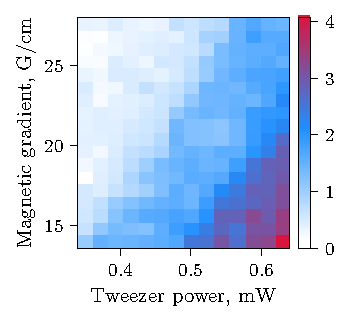
\includegraphics{fig-py/step-plot-2d.pdf}
    \caption{
        Measured 2D step plot as a function of tweezer power and magnetic field gradient. Each point indicates the average atom number obtained for a given combination of parameters. This map confirms that for any spill power, a suitable magnetic gradient can be found to achieve a desired quantized atom number.
    }
    \label{fig:spillingadd-2d}
\end{figure}



\begin{figure}
    \centering
    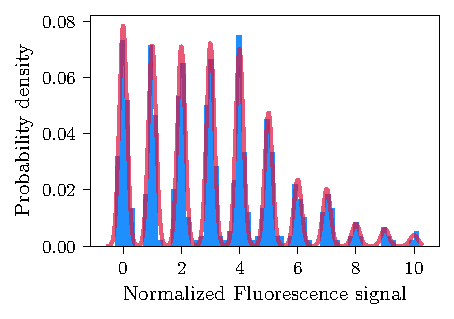
\includegraphics{fig-py/atom-counting.pdf}
    \caption{
        Calibration histogram for single-atom counting based on fluorescence signal after after loading to the MOT. Clear quantized peaks correspond to integer atom numbers; the solid red line is a multi-Gaussian fit to the distribution. 
    }
    \label{fig:spillingadd}
\end{figure}



% \begin{figure}
%     \centering
%     \addletter{145}{a}
%     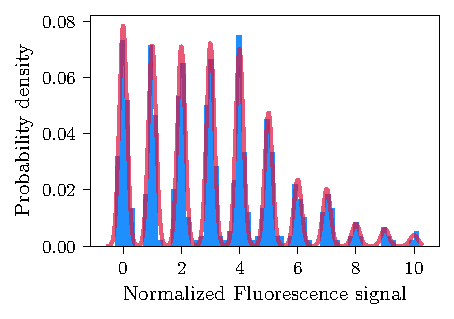
\includegraphics{fig-py/atom-counting.pdf}
%     \phantom{4242}
%     \addletter{145}{b}
%     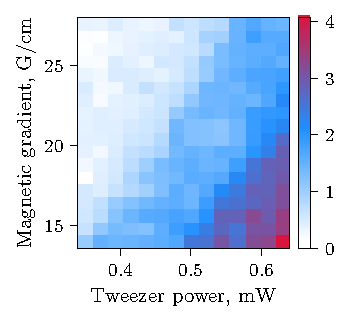
\includegraphics{fig-py/step-plot-2d.pdf}
%     \caption{
%         (a) Calibration histogram for single-atom counting based on fluorescence signal after after loading to the MOT. Clear quantized peaks correspond to integer atom numbers; the solid red line is a multi-Gaussian fit to the distribution. 
%         (b) Measured 2D step plot as a function of tweezer power and magnetic field gradient. Each point indicates the average atom number obtained for a given combination of parameters. This map confirms that for any spill power, a suitable magnetic gradient can be found to achieve a desired quantized atom number.
%     }
%     \label{fig:spillingadd}
% \end{figure}

% \textbf{From frequency to position}. И в camera based balancing, и в atoms based balancing для обработки изображений удобно определить афинное преобразование из frequency space to position space:
% \begin{equation*}
% 	\vc{r} = H \vc{\omega}
% 	\hspace{5 mm} \leftrightarrow \hspace{5 mm} 
% 	\begin{pmatrix}
% 		x \\ y
% 	\end{pmatrix} = \begin{pmatrix}
% 		h_{11} & h_{12} & h_{13} \\
% 		h_{21} & h_{22} & h_{23} \\
% 	\end{pmatrix} 
% 	\begin{pmatrix}
% 		\sub{\omega}{hor} \\
% 		\sub{\omega}{ver} \\
% 		1
% 	\end{pmatrix}.
% \end{equation*}
% Можно, например, для случайных $\vc{\omega}_j \in [\sub{\omega}{min},\, \sub{\omega}{max}]$ измерить $\vc{r}_j$, таким образом сформировав две матрицы $\omega_{ij}$ with $i \in \{\mathrm{hor},\, \mathrm{ver}\}$ and $r_{ij}$ with $i \in \{x, y\}$. Остается решить уравнение на $H$ (что соответсвует Least squares method):
% \begin{equation}
% 	r = H \omega,
% 	\hspace{0.5cm} \Rightarrow \hspace{0.5cm}
% 	r \omega\T = H \omega \omega\T
% 	\hspace{0.5cm} \Rightarrow \hspace{0.5cm}
% 	r \omega\T \left(\omega \omega\T\right)^{-1} = H.
% 	\label{LinReg:freq2pos}
% \end{equation}